% Current methodology for the default empirical model and backtest comparison.
% Standalone: no external figures or project dependencies.
\documentclass[11pt,a4paper]{article}
\usepackage[T1]{fontenc}
\usepackage{lmodern}
\usepackage[margin=24mm]{geometry}
\usepackage{amsmath,amssymb,microtype}
\usepackage{booktabs,tabularx,array,xcolor,hyperref}
\usepackage{tikz}
\usetikzlibrary{arrows.meta,positioning,calc}
\definecolor{capacitygreen}{HTML}{176B57}
\hypersetup{colorlinks=true,linkcolor=capacitygreen,urlcolor=capacitygreen,citecolor=capacitygreen,
 pdftitle={Capacity Lab: Objectives, Approaches and Calibration},pdfauthor={Capacity Lab}}
\setlength{\parindent}{0pt}
\setlength{\parskip}{6pt}
\setlength{\emergencystretch}{2em}
\renewcommand{\arraystretch}{1.2}
\newcolumntype{L}{>{\raggedright\arraybackslash}X}
\begin{document}
\begin{center}
{\LARGE\bfseries Capacity Lab\par}
\vspace{3mm}
{\large Objectives, Approaches and Calibration\par}
\vspace{2mm}
15 October 2026
\end{center}

\section{Objective of the exercise}
Estimate how a strategy's net performance changes as assets under management (AUM) grow, and identify the AUM at which its net information ratio (IR) reaches a chosen minimum. The exercise supports capacity planning: it explains the assumptions behind an indicated capacity, rather than treating capacity as a single fixed property of the strategy.

The dashboard reports net IR, annual net alpha and the AUM associated with the minimum-IR and zero-IR thresholds. IR is net alpha divided by tracking error. Use the same return horizon and risk conventions when comparing results.

\textbf{Two AUM references have different jobs.} Current AUM anchors historical trading observations. In universe mode, scenario order size is derived from AUM, turnover and the annual order count; stock ADV stays fixed. USD 0.5bn is the starting point of the calibrated net-IR curve. The sampler preview defaults to current AUM; the empirical curve starts at USD 0.5bn.

\section{Two complementary approaches}
\subsection{Empirical approach}
The \textbf{Empirical IR curve} combines observed trading and liquidity inputs with three calibrated model pillars: impact costs, alpha decay and transfer-coefficient (TC) decay. It answers: \emph{what happens to performance if orders grow and the chosen execution and implementation assumptions hold?}

Trading observations inform the impact-cost pillar. Alpha-decay and TC points are user estimates; they are not automatically inferred from trade history. The approach makes these assumptions visible and lets users adjust them in Model Calibration.

\subsection{Backtest approach}
The \textbf{Backtest IR curve} fits a decreasing power curve to AUM and IR observations from optimised historical backtests. It provides a separate estimate of capacity based on the strategy's behaviour in those backtests.

Use comparable observations: the same investment period, risk conventions and cost definitions. The fitted curve can be adjusted in the sidebar. Illustrative dashboard observations must be replaced before treating this comparison as historical evidence.

\textbf{Read the approaches together.} Summary compares their current IR and capacity thresholds. Differences can reveal assumptions that need review. The two curves remain separate; the dashboard does not average them or use the backtest fit to calibrate the empirical pillars.

\newpage
\section{Empirical approach: inputs, pillars and calibration}
\subsection{Inputs}
Start in \textbf{Inputs \& strategy}. Confirm the universe ADV percentiles and annual parent-order count, and check that historical bucket observations correspond to current AUM.

\begin{tabularx}{\textwidth}{@{}p{.27\textwidth}L@{}}
\toprule
Input & Purpose and units \\
\midrule
Current AUM & Historical order-size reference; USD billions. \\
ADV percentiles & Locally saved USD daily ADV boundaries; interpolate to approximate a 300-stock universe. \\
Annual parent orders & Default 971 across four quarters, about 81 per month. \\
Historical ADV buckets & Ratios and estimated costs for fitting; counts and notionals for comparison. \\
Estimated bucket impact & Positive cost in basis points (bp) per traded dollar. \\
One-way annual turnover & Twice this fraction gives annual traded value / AUM. \\
Tracking error & Fixed annual active-return risk, entered in percent. \\
Calibration triples & Three points each for alpha decay and TC. \\
Minimum net IR & Performance threshold used to indicate capacity. \\
\bottomrule
\end{tabularx}

Alternatively, upload actual parent orders with positive \texttt{q} (order notional) and \texttt{adv} (average daily traded value) in the same currency. The CSV supplies order sizes and liquidity; estimated bucket costs still supply the impact-curve calibration.

\subsection{Three model pillars}
\subsubsection{Impact costs: larger orders are more expensive to trade}
The \textbf{ADV bucket sampler} automatically fits a nonnegative power cost curve to the estimated bucket impacts. There are no per-bucket sliders or manual impact-fit controls. Each bucket has equal weight in fitting; aggregate portfolio costs use traded-notional weights.

\textbf{Generate orders from the stock universe.} Interpolate the locally saved ADV boundaries in log USD at 300 equally spaced midpoint stock ranks. This approximates individual stock ADVs; it does not recover the original stock observations. Each stock has equal selection probability and can be selected repeatedly.

For $N=971$ annual orders, one-way turnover fraction $T$ and AUM $A$ in USD billions, the equal ticket is $q(A)=2TA10^9/N$ USD. Order/ADV is $q(A)/ADV_i$. Each annual book therefore trades exactly twice one-way turnover times AUM. At USD 3.4bn and 13.90\% turnover, each ticket is USD 973,429.45. Trade count and turnover are editable; timing within quarters is not simulated.

The stock ADVs generate the buckets. Reuse the same stock selections at current AUM, twice current AUM and three times current AUM, scaling tickets with AUM while ADV stays fixed. An overflow bucket retains orders above 100\% ADV. Historical bucket frequencies are a diagnostic, not a calibration target.

Annual cost in bp is average impact multiplied by twice one-way turnover. Equal tickets make count and notional weights identical; CSV mode preserves actual notionals. Nonlinear impact has an empirical literature~\cite{almgren}, but this specific fit remains a scenario estimate, especially outside the observed participation range.

\newpage
\subsubsection{Alpha decay: execution congestion reduces performance}
Users specify three \textbf{(AUM, percentage of trades taking more than one day, net IR)} points. The dashboard fits two linked power curves: AUM to multi-day trade percentage, then multi-day trade percentage to IR. Their curvatures are inferred automatically.

The starting point is USD 0.5bn with zero multi-day trades. The default assumptions are:
\begin{center}
\begin{tabular}{rrr}
\toprule
AUM (USD bn) & Trades taking $>1$ day & Net IR \\
\midrule
0.50 & 0.00\% & 0.60 \\
3.00 & 2.00\% & 0.57 \\
6.00 & 10.00\% & 0.50 \\
\bottomrule
\end{tabular}
\end{center}
These points isolate alpha decay while other effects are held fixed. Multi-day percentage counts parent orders equally, regardless of notional or forecast strength. It summarises congestion without distinguishing, for example, two-day and ten-day orders.

\subsubsection{Transfer coefficient: implementation efficiency declines}
Users specify three \textbf{(TC, AUM, annual alpha)} points. The dashboard fits power curves from AUM to TC, then TC to annual alpha. In this exercise, alpha means annual net alpha with other effects fixed.

The default assumptions are:
\begin{center}
\begin{tabular}{rrr}
\toprule
TC & AUM (USD bn) & Annual alpha \\
\midrule
60.00\% & 0.50 & 1.00\% \\
40.00\% & 3.00 & 0.60\% \\
25.00\% & 6.00 & 0.30\% \\
\bottomrule
\end{tabular}
\end{center}
The combined model uses this alpha relationship as a \textbf{relative retention factor}: divide calibrated alpha at each AUM by its initial value. The defaults therefore retain 100.00\%, 60.00\% and 30.00\% of the TC-related alpha at the three AUM points. It does not use the raw TC ratio as the retention factor.

These triples imply nonlinear AUM-to-TC decay and a linear TC-to-alpha link. Other triples can imply different curvature. The initial 1.00\% is a normalising reference, not a second absolute alpha anchor added to the combined model.

\newpage
\subsection{Calibration workflow}
\begin{enumerate}
\item Confirm current AUM and the observed orders or buckets in Inputs \& strategy. Check estimated impact costs, tracking error and turnover.
\item In Model Calibration, inspect the automatically fitted impact curve and the trading-book distribution. Change AUM, sample count, seed or turnover as needed.
\item Edit the three alpha-decay points and review both linked relationships. AUM points use USD 0.5bn increments; percentages must increase and IR must decrease.
\item Edit the three TC points. AUM must increase, while TC and annual alpha must decrease. Review the resulting retention factor.
\item Review Empirical IR curve and Summary. In the default combined model, calibration edits update both immediately. Save through Inputs \& strategy to persist the chosen inputs and settings.
\end{enumerate}

\subsection{How the pillars combine}
Start with the alpha-decay IR, multiply by TC-alpha retention, and deduct \textbf{only the increase in impact costs above USD 0.5bn}:
\[
\boxed{IR(A)=I_{\alpha}(A)\,H_{TC}(A)-\Delta C_{IR}(A).}
\]
Here $I_\alpha$ is the calibrated alpha-decay IR, $H_{TC}$ is the TC-alpha retention factor and $\Delta C_{IR}$ is incremental annual impact cost expressed in IR units. The initial net-IR point already includes baseline costs, so the full baseline cost is not deducted again.

With the default points, IR before incremental impact costs is $0.57\times0.60=0.342$ at USD 3bn and $0.50\times0.30=0.150$ at USD 6bn. Net IR at USD 0.5bn remains exactly 0.60. Annual net alpha in percent equals net IR multiplied by tracking error in percent.

\subsection{Reading the results}
\textbf{Empirical IR curve} shows net IR and net alpha across AUM. \textbf{Summary} compares empirical and backtest capacity indications, and separates the empirical decline into alpha-decay, TC and incremental-impact contributions.

Capacity is the first AUM from USD 0.5bn where the central curve reaches the selected threshold. A threshold not reached within the displayed range does not imply unlimited capacity. Projections beyond calibration points are labelled extrapolation. The combined domain stops when either retained-alpha factor first reaches zero, or at an earlier pillar-domain limit.

The default is \textbf{Deterministic}: a central curve without intervals. Select \textbf{Monte Carlo} for conditional 5th--95th percentile ranges. Tables display at most two decimals; calculations, saved values and CSV exports preserve full precision.

\newpage
\appendix
\section{Simulation assumptions and calculation notes}
\subsection{What Monte Carlo samples}
A sample is an alternative trading book and congestion outcome, not a draw of an individual trade's alpha forecast. The diagram follows one simulation through the model. The cost and congestion paths use independent random draws.

\begin{center}
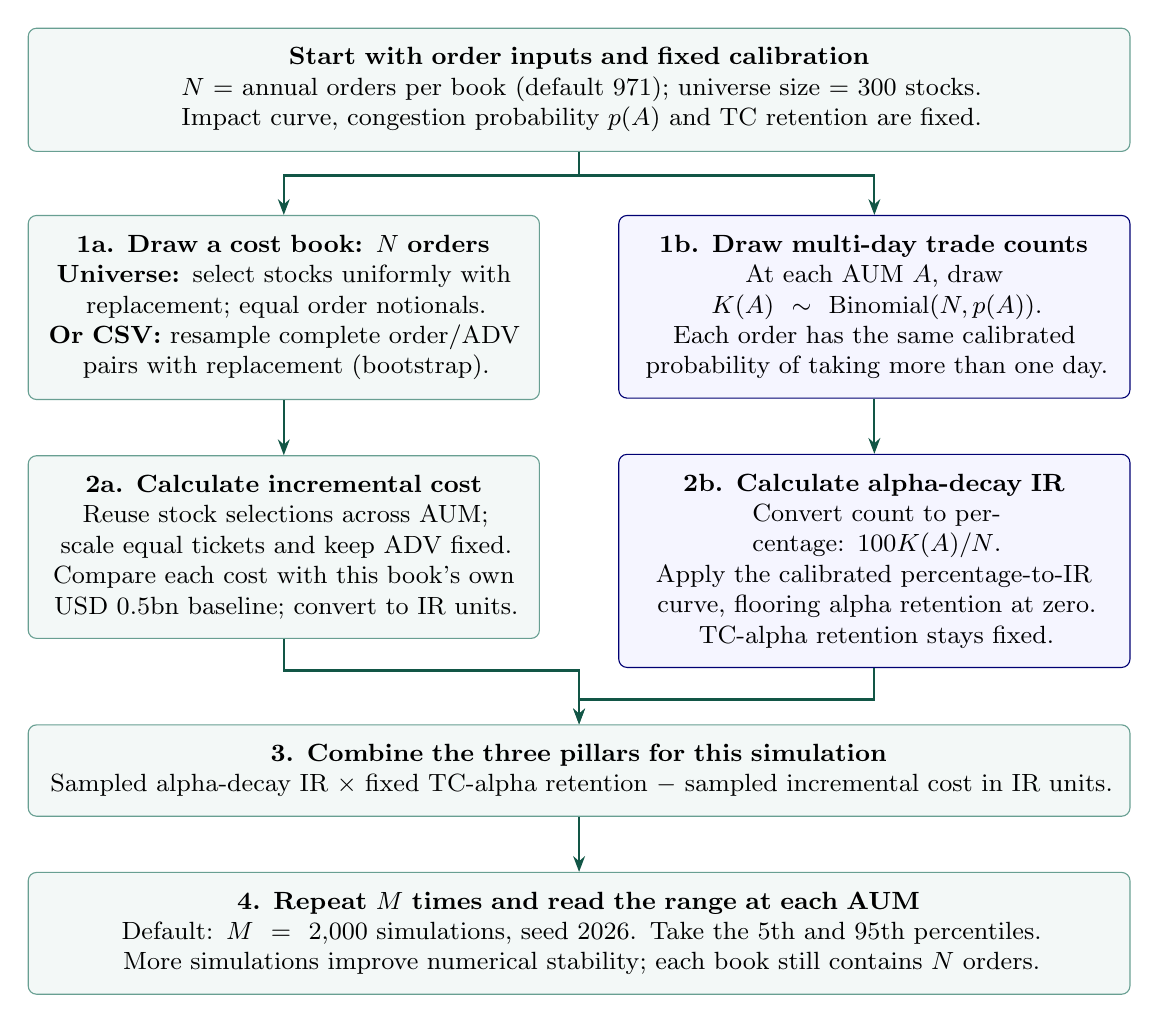
\begin{tikzpicture}[
 box/.style={draw=capacitygreen!65,rounded corners=3pt,fill=capacitygreen!5,
 text width=6.0cm,align=center,inner sep=7pt,font=\small},
 bluebox/.style={box,draw=blue!45!black,fill=blue!4},
 wide/.style={box,text width=13.5cm},
 flow/.style={-{Stealth[length=2mm]},thick,draw=capacitygreen!80!black}]
\node[wide] (setup) {\textbf{Start with order inputs and fixed calibration}\\
$N$ = annual orders per book (default 971); universe size = 300 stocks.\\
Impact curve, congestion probability $p(A)$ and TC retention are fixed.};
\node[box,below=8mm of setup.south west,anchor=north west] (book) {
\textbf{1a. Draw a cost book: $N$ orders}\\
\textbf{Universe:} select stocks uniformly with replacement; equal order notionals.\\
\textbf{Or CSV:} resample complete order/ADV pairs with replacement (bootstrap).};
\node[bluebox,below=8mm of setup.south east,anchor=north east] (congestion) {
\textbf{1b. Draw multi-day trade counts}\\
At each AUM $A$, draw\\
$K(A)\sim\mathrm{Binomial}(N,p(A))$.\\
Each order has the same calibrated probability of taking more than one day.};
\node[box,below=7mm of book] (cost) {\textbf{2a. Calculate incremental cost}\\
Reuse stock selections across AUM; scale equal tickets and keep ADV fixed.\\
Compare each cost with this book's own USD 0.5bn baseline; convert to IR units.};
\node[bluebox,below=7mm of congestion] (alpha) {\textbf{2b. Calculate alpha-decay IR}\\
Convert count to percentage: $100K(A)/N$.\\
Apply the calibrated percentage-to-IR curve, flooring alpha retention at zero.\\
TC-alpha retention stays fixed.};
\coordinate (mid) at ($(cost.south)!0.5!(alpha.south)$);
\node[wide,below=9mm of mid] (combine) {\textbf{3. Combine the three pillars for this simulation}\\
Sampled alpha-decay IR $\times$ fixed TC-alpha retention $-$ sampled incremental cost in IR units.};
\node[wide,below=7mm of combine] (repeat) {\textbf{4. Repeat $M$ times and read the range at each AUM}\\
Default: $M=2{,}000$ simulations, seed 2026. Take the 5th and 95th percentiles.\\
More simulations improve numerical stability; each book still contains $N$ orders.};
\draw[flow] (setup.south) -- ++(0,-3mm) -| (book.north);
\draw[flow] (setup.south) -- ++(0,-3mm) -| (congestion.north);
\draw[flow] (book) -- (cost);
\draw[flow] (congestion) -- (alpha);
\draw[flow] (cost.south) -- ++(0,-4mm) -| (combine.north);
\draw[flow] (alpha.south) -- ++(0,-4mm) -| (combine.north);
\draw[flow] (combine) -- (repeat);
\end{tikzpicture}
\end{center}
{\small\textbf{Figure 1. Sampling workflow.} Only the cost book is reused across AUM. The separate congestion counts do not track the same individual trades across the curve. The displayed central curve uses calibrated congestion and mean simulated impact; it is not the mean of the simulated final IR outcomes.}

\textbf{Where do buckets come from?} Each sampled stock's ADV and the equal ticket determine order/ADV. Reclassify these ratios at each AUM; do not draw from historical bucket shares. Uniform stock selection is equivalent to multinomial stock counts with probabilities $1/300$. Binomial and multinomial sampling are standard count models~\cite{agresti}; CSV resampling is the empirical bootstrap~\cite{efron}. The seed makes draws reproducible.

\newpage
\subsection{Interpretation and limitations}
For alpha-decay purposes, orders are exchangeable: the model has no trade-specific alpha forecasts or delay sensitivities. This is a count-based approximation, not an explicit allocation of equal alpha dollars to every trade. Cost aggregation remains notional-weighted; in universe mode this equals count weighting because tickets are equal.

Congestion-count draws and cost composition are independent in the simulation. In reality, difficult-to-execute trades may carry more or less alpha. The ranges exclude this dependence, calibration uncertainty, clustered orders and changes in market liquidity. The universe sampler also assumes uniform stock selection, equal tickets and a percentile-derived ADV approximation; it does not reproduce historical bucket frequencies by construction. They are conditional pointwise ranges, not simultaneous confidence bands or guarantees of future performance. The centre curve uses the calibrated congestion share and mean simulated impact, not the mean of the nonlinear final outcomes. Ranges collapse at the USD 0.5bn anchor.

The Fundamental Law of Active Management motivates separating forecast skill, independent breadth and implementation efficiency. This dashboard does not estimate skill or independent breadth, and its TC scenario is not an estimated forecast-to-position correlation~\cite{grinold,clarke}.

\subsection{Units and fitted relationships}
AUM is in USD billions. Order/ADV is a fraction internally and a percentage in the interface. Annual alpha and tracking error use percentage points. If $C(A)$ is annual portfolio cost in bp and $TE$ is tracking error in percent, incremental cost in IR units is
\[
\Delta C_{IR}(A)=\frac{C(A)-C(0.5)}{100\,TE}.
\]
\subsection{Academic foundations and model choices}
The references support the sampling methods and the economic motivation for the pillars. Efron describes the bootstrap~\cite{efron}; Agresti covers binomial and multinomial count models~\cite{agresti}. Almgren and co-authors study nonlinear market impact~\cite{almgren}. G\^arleanu and Pedersen analyse trading with decaying return predictors and transaction costs~\cite{garleanu}. Grinold and Clarke and co-authors provide the active-management and implementation-efficiency context~\cite{grinold,clarke}.

\textbf{What the literature does not establish here.} Our uniform stock selection, equal tickets, interpolated ADV universe, three calibration points, fitted congestion-to-IR curve, TC-alpha retention mapping, independence of the two random paths and multiplicative combination are choices for this dashboard. The cited works do not validate these choices or turn the simulated percentile ranges into full forecast confidence intervals.

\newpage
\begin{thebibliography}{9}
\bibitem{agresti} Agresti, A. (2002).
Introduction: Distributions and Inference for Categorical Data.
In \emph{Categorical Data Analysis}, 2nd ed., Chapter 1. Wiley.
\href{https://doi.org/10.1002/0471249688.ch1}{doi:10.1002/0471249688.ch1}.

\bibitem{efron} Efron, B. (1979).
Bootstrap Methods: Another Look at the Jackknife.
\emph{The Annals of Statistics}, 7(1), 1--26.
\href{https://doi.org/10.1214/aos/1176344552}{doi:10.1214/aos/1176344552}.

\bibitem{almgren} Almgren, R., Thum, C., Hauptmann, E., and Li, H. (2005).
\emph{Direct Estimation of Equity Market Impact}.
Working paper, 10 May 2005.
\href{https://www.cis.upenn.edu/~mkearns/finread/costestim.pdf}{Full paper (University of Pennsylvania)}.

\bibitem{garleanu} G\^arleanu, N., and Pedersen, L. H. (2013).
Dynamic Trading with Predictable Returns and Transaction Costs.
\emph{The Journal of Finance}, 68(6), 2309--2340.
\href{https://doi.org/10.1111/jofi.12080}{doi:10.1111/jofi.12080}.

\bibitem{grinold} Grinold, R. C. (1989).
The Fundamental Law of Active Management.
\emph{The Journal of Portfolio Management}, 15(3), 30--37.
\href{https://doi.org/10.3905/jpm.1989.409211}{doi:10.3905/jpm.1989.409211}.

\bibitem{clarke} Clarke, R. G., de Silva, H., and Thorley, S. (2002).
Portfolio Constraints and the Fundamental Law of Active Management.
\emph{Financial Analysts Journal}, 58(5), 48--66.
\href{https://doi.org/10.2469/faj.v58.n5.2468}{doi:10.2469/faj.v58.n5.2468}.
\end{thebibliography}
\end{document}
